\documentclass[11pt]{article}
\usepackage[utf8]{inputenc}
\usepackage[T1]{fontenc}
\usepackage{lmodern}
\usepackage{geometry}
\usepackage{tikz}
\usetikzlibrary{arrows.meta,shapes.geometric}

\geometry{paperwidth=16cm,paperheight=6.6cm,margin=0cm}
\pagestyle{empty}
\setlength{\parindent}{0pt}

\definecolor{ctxFill}{RGB}{238,242,245}
\definecolor{ctxLine}{RGB}{155,168,179}
\definecolor{ctxText}{RGB}{38,52,67}
\definecolor{exFill}{RGB}{220,233,247}
\definecolor{exLine}{RGB}{23,54,93}
\definecolor{prFill}{RGB}{200,240,236}
\definecolor{prLine}{RGB}{8,127,140}
\definecolor{prText}{RGB}{6,79,87}

\begin{document}
\noindent
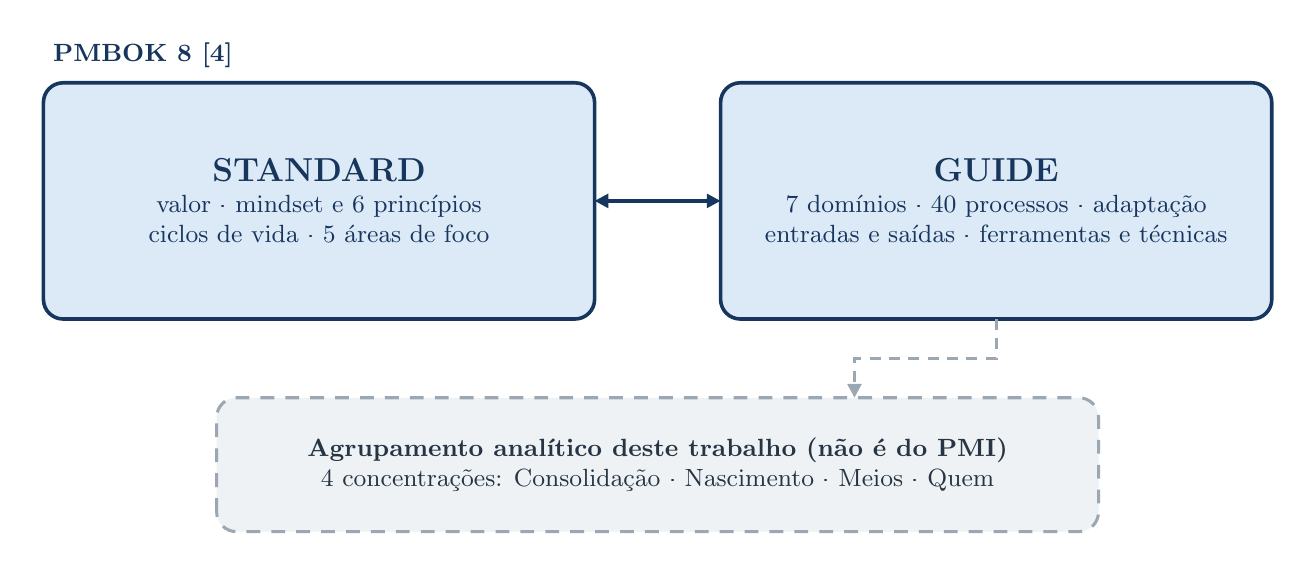
\begin{tikzpicture}[x=1cm,y=1cm,font=\small]
  \path[use as bounding box] (0,0) rectangle (16,6.6);
  \node[anchor=west,text=exLine] at (0.2,6.25) {\textbf{PMBOK 8 [4]}};
  \draw[fill=exFill,draw=exLine,line width=1.3pt,rounded corners=0.25cm] (0.2,2.9) rectangle (7.2,5.9);
  \draw[fill=exFill,draw=exLine,line width=1.3pt,rounded corners=0.25cm] (8.8,2.9) rectangle (15.8,5.9);
  \node[align=center,text=exLine] at (3.7,4.4) {\large\textbf{STANDARD}\\ valor · mindset e 6 princípios\\ciclos de vida · 5 áreas de foco};
  \node[align=center,text=exLine] at (12.3,4.4) {\large\textbf{GUIDE}\\ 7 domínios · 40 processos · adaptação\\entradas e saídas · ferramentas e técnicas};
  \draw[draw=exLine,line width=1.2pt,{Triangle[length=5pt,width=5pt]}-{Triangle[length=5pt,width=5pt]}] (7.2,4.4) -- (8.8,4.4);
  \draw[fill=ctxFill,draw=ctxLine,line width=1.1pt,dash pattern=on 5pt off 4pt,rounded corners=0.25cm] (2.4,0.2) rectangle (13.6,1.9);
  \node[align=center,text=ctxText] at (8.0,1.05) {\textbf{Agrupamento analítico deste trabalho (não é do PMI)}\\ 4 concentrações: Consolidação · Nascimento · Meios · Quem};
  \draw[draw=ctxLine,line width=1.1pt,dash pattern=on 4pt off 3pt,-{Triangle[length=5pt,width=5pt]}] (12.3,2.9) -- (12.3,2.4) -- (10.5,2.4) -- (10.5,1.9);
\end{tikzpicture}
\end{document}
